\documentclass{homework}
\title{Homework 6}
\begin{document}
\maketitle

\begin{problem} This is basically trigonometry.
Let \(\ell_i(x) = \prod_{j\ne i} (x-x_j)/\prod_{j\ne i}(x_i-x_j)\). We set the constant \(\lambda_i = 1/\prod_{j\ne i}(x_i - x_j)\), then for Chebyshev nodes we already know that
\[\lambda_i = \begin{cases}
\frac{2^{N-1}}{N}(-1)^i & (0 < i < N)\\
\frac{2^{N-2}}{N}(-1)^i & (i = 0, N).
\end{cases}\]
The entries of the differentiation matrix is
\begin{align*}
D_{ij} &= \ell'_j(x_i)\\
&= \lambda_j \left. \frac{\d}{\d[x]} \prod_{k\ne j} (x - x_k) \right|_{x = x_i}\\
&= \lambda_j \sum_{k \ne j}\prod_{\substack{l \ne k\\l\ne j}} (x_i - x_l).
\end{align*}
When \(i\ne j\), the only term that doesn't vanish is \(\prod_{l\ne i, l\ne j} (x_i - x_l)\). We substitute in \(x_k = \cos \frac{k\pi}{N}\), and rearrange the factors. First we assume \(i\ne 0,N\).
\begin{align*}
&\quad \prod_{\substack{l\ne i\\l\ne j}} \left[\cos \frac{i\pi}{N} - \cos\frac{l\pi}{N}\right]\\
&= \prod_{\substack{l\ne i\\l\ne j}} (-2)\sin\frac{(i+l)\pi}{2N}\sin\frac{(i-l)\pi}{2N}\\
&= (-1)^{N-i}(-2)^{N-1} \sin\frac{i\pi}{2N}\sin\frac{(i-N)\pi}{2N}\left.\prod_{u=1}^{2N-1} \sin \frac{u\pi}{2N} \right/ \sin\frac{2i\pi}{2N} \sin\frac{(i+j)\pi}{2N}\sin\frac{(i-j)\pi}{2N}\\
&=-\frac{(-1)^{N-i}(-2)^{N-1} \sin\frac{2i\pi}{2N}/2 \cdot 2N \cdot 2^{-2N+1}}{\sin\frac{2i\pi}{2N} \sin\frac{(i+j)\pi}{2N}\sin\frac{(i-j)\pi}{2N}}\\
&= \frac{(-1)^{i}N}{2^{N} (\cos\frac{i\pi}{N} - \cos\frac{j\pi}{N})} = \frac{1}{\lambda_i(x_i - x_j)}.
\end{align*}
Here we used the well-known identity that \(\prod_{j=1}^{n-1}\sin\frac{j\pi}{n} = n2^{-n+1}\). After multiplying with \(\lambda_j\) it is as desired. When \(i = 0\), the expression becomes
\begin{align*}
\prod_{l=1, l\ne j}^{N} 2 \sin^2\frac{l\pi}{2N}
&= 2^{N-1}\left[ \prod_{l=1}^{N-1}\sin\frac{l\pi}{2N} \middle/ \sin\frac{j\pi}{2N} \right]^2\\
&=2^{N-1} \left.\prod_{k=1}^{2N-1} \sin\frac{k\pi}{2N} \right/ \sin^2\frac{j\pi}{2N}\\
&= \frac{2^{N-1} \cdot 2N \cdot 2^{-2N+1}}{ \sin^2 \frac{j\pi}{2N}} \\
&= \frac{N}{2^{N-2}(1-\cos \frac{j\pi}{N})} = \frac{1}{\lambda_i(x_i - x_j)},
\end{align*}
which is also as desired. When \(i = j\), we have
\[D_{ii} = \frac{\sum_{k\ne i} \prod_{l\ne k, l\ne i} (x_i - x_l)}{\prod_{l\ne i}(x_i - x_l)} = \sum_{k\ne i} \frac{1}{x_i - x_k}.\]
Consider the polynomial \(p_i(x) = \ell(x_i - x)\). Its roots are exactly \(x_i - x_k\) and \(0\). Therefore after dividing by \(x\), \(p_i(x)/x\) has no zero root, and by Vieta's theorem, the sum of its reciprocal roots is
\[\sum_{k\ne i}\frac{1}{x_i - x_k} = -\frac{c_{i,2}}{c_{i,1}} = -\frac{p_i''(0)}{2p_i'(0)} = \frac{\ell''(x_i)}{2\ell'(x_i)}\]
where \(c_{i,n}\) is the \(n\)-th coefficient of \(p_i(x)\). We use the trigonometric expression of
\[\ell(x) = \frac{\sin(N\arccos x)}{\sin\arccos x},\]
obtaining
\[\ell'(x) = \frac{x\sin(N\arccos x)}{(1-x^2)^{3/2}}-\frac{N\cos(N\arccos x)}{1-x^2},\]
and the second derivative \(\ell''(x)\)
\[\frac{(N^{2} x^{2} - N^{2} + 2 x^{2} + 1)\sin(N\arccos x) - 3 N x \sqrt{1 - x^{2}} \cos{(N\arccos x)}}{(1-x^2)^{5/2}}.\]
Substituting \(x_i = \cos\frac{i\pi}{N}\), we have for \(i \ne 0,N\), the \(\sin(N\arccos x)\) terms vanish, and we are left with
\[D_{ii} = -\frac{x_i}{2(1-x_i^2)}.\] For \(i=0\), the above method faces the difficulty of division by zero, but we can directly compute
\begin{align*}
D_{00} &= \sum_{k=1}^N \frac{1}{1-\cos\frac{k\pi}{N}}\\
&= \frac12 + \sum_{k=1}^{N-1} \frac{1}{2\sin^2\frac{k\pi}{2N}}\\
&= \frac12 + \frac12 \sum_{k=1}^{N-1} \left[1 + \cot^2 \frac{k\pi}{2N}\right]\\
&= \frac N2 + \frac12 \sum_{k=1}^{N-1} \cot^2 \frac{k\pi}{2N} = \frac{N}{2}+ \frac{(N-1)(2N-1)}{6},
\end{align*}
where the last identity is well known. This simplifies to the desired result. The \(i=N\) case is symmetric. We covered all the cases, and verified that in each case the coefficients are as given in the slides.
\end{problem}

\begin{problem}
We use a rudimentary error estimator:
\[I \approx 2I(h/2) - I(h),\]
where \(I(h)\) is the integral evaluated at step size \(h\). This gives an error estimate \(E(h)\). But since we already evaluated \(I(h/2)\), we use this more accurate integral, and the resulting error estimate is
\[E(h/2) = \left|I(h) - I(h/2) \right|.\]
We evaluated the integral recursively: First we directly use the static rule on the whole interval. If the error estimate is already lower than the tolerance, we stop and return the result. Otherwise, we bisect the interval, and half the tolerance for each subinterval.

This results in a very simple adaptive algorithm. We test it on
\[\int_{10^{-8}}^1 \sqrt x \log x+ \sin(10x) \d[x]\]
and
\[\int_0^{10} \sin x^2 \d[x].\]
This gives rather nice results.
\begin{center}
\begin{tabular}{c c c}
Tolerance & Simpson & Newton\\\hline
\(10^{-6}\) & \(1.280 \times 10^{-9}\) & \(1.210 \times 10^{-10}\)\\
\(10^{-9}\) & \(1.402 \times 10^{-12}\) & \(2.230 \times 10^{-12}\)\\
\(10^{-12}\) & \(1.619 \times 10^{-15}\) & \(1.221 \times 10^{-15}\)\\[1ex]
\(10^{-6}\) & \(1.937 \times 10^{-9}\) & \(5.379 \times 10^{-10}\)\\
\(10^{-9}\) & \(4.773 \times 10^{-12}\) & \(2.447 \times 10^{-12}\)\\
\(10^{-12}\) & \(8.882 \times 10^{-16}\) & \(1.110 \times 10^{-16}\)\\
\end{tabular}
\end{center}
A quick debug session shows that in the second integral, the divided intervals indeed get denser and denser towards the right, where the function oscillates more.
\end{problem}

\begin{problem} We have already derived the orders of errors for the first two schemes, which are \(Mh + \epsilon/h\) and \(Mh^2 + \epsilon/h\), respectively. Note that we should be able to slightly improve accuracy, by using \((x+h)-x\) instead of \(h\) in the denominator, since for small \(h\), the argument of \(f\) would not be exactly \(x+h\) due to rounding errors. So by using the same number in the denominator we can get a more accurate result. The same holds for the second scheme. These are plotted as a bonus in the results.

For the third scheme, the rounding error is bounded by \(\epsilon/h\) too, where \(\epsilon\) is the maximum of the rounding errors of \(f(x-2h), f(x-h),f(x+h)\) and \(f(x+2h)\). For the truncation error, we Taylor expand to get
\[f(x+\eta) = f(x) + f'(x) \eta + \frac12f''(x)\eta^2 + \frac16 f'''(x)\eta^3. + \frac1{24}f''''(x)\eta^4 + \frac1{120} f'''''(\xi)\eta^5.\]
Therefore
\[f(x-2h) -8f(x-h) + 8f(x+h) - f(x+2h)
=12 f'(x)h + \frac{2}{5}M_5 h^5,\]
where \(|M_5| \le \sup_{|\eta| \le 2h} |f'''''(x+\eta)|\). So dividing by \(12h\), the truncation error is \(\frac{1}{30} M_5 h^4\). This gives a total error of \[E(h) = \frac{M_5}{30}h^4 + \frac{\epsilon}{h}.\]

The code is trivial, see the appendix. We can see that the initial errors almost exactly follow \(h, h^2, h^4\) respectively by looking at the slope of the line, confirming our truncation error analysis. When \(h\) is small, the curves tend to join and follow \(\epsilon/h\), where \(\epsilon\) is around \(10^{-16}\), the machine precision. The best accuracy is obtained at around \(\sqrt\epsilon, \sqrt[3]\epsilon, \sqrt[5]\epsilon\), respectively.
\begin{center}
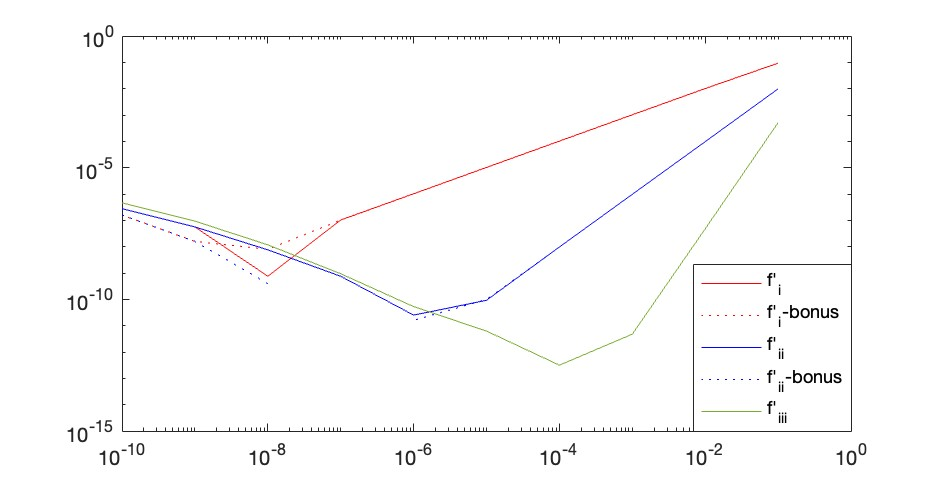
\includegraphics[width=0.7\textwidth]{Hw6-Fig2.jpg}
\end{center}
The bonus schemes do slightly improve (one of the datapoints reached zero error) the accuracy, but not by a great factor.
\end{problem}

\newpage
\section*{Appendix: Souce Code}
Code can also be found at 
\begin{center}
\texttt{https://github.com/Trebor-Huang/Numerical-Analysis-Homework}
\end{center}
\matlabfile{Hw6.m}
\lstinputlisting[
    language=Python,
    frame=single,
    basicstyle=\small\ttfamily,
    escapechar=`
]{Hw6.py}
\end{document}
